\documentclass[10pt]{article}
\usepackage{tmlr}
% For a de-anonymised preprint use: \usepackage[preprint]{tmlr}

\usepackage[utf8]{inputenc}
\usepackage{amsmath,amssymb,amsthm}
\usepackage{booktabs}
\usepackage{multirow}
\usepackage{graphicx}
\usepackage{xcolor}
\usepackage{algorithm}
\usepackage{algpseudocode}
\usepackage{hyperref}
\usepackage{url}
\usepackage{cleveref}
\setlength{\belowcaptionskip}{4pt}  % tables have captions above

\newtheorem{proposition}{Proposition}
\newtheorem{definition}{Definition}
\newtheorem{remark}{Remark}

\newcommand{\R}{\mathbb{R}}
\newcommand{\E}{\mathbb{E}}
\newcommand{\shd}{\mathrm{SHD}}
\newcommand{\psidag}{$\psi$DAG}
\newcommand{\psidbn}{$\psi$DBN}
\newcommand{\feddbn}{fedDBN}
\newcommand{\exdbn}{ExDBN}
\newcommand{\todo}[1]{\textcolor{red}{[TODO: #1]}}

\title{fedDBN: Federated Learning of Dynamic Bayesian Networks\\and the Price of Federation}

\author{\name Anonymous authors \\ \addr Paper under double-blind review}

\def\month{MM}
\def\year{YYYY}
\def\openreview{\url{https://openreview.net/forum?id=XXXX}}

\begin{document}
\maketitle

\begin{abstract}
We study learning linear dynamic Bayesian networks (structural vector autoregressions with an
acyclic contemporaneous graph) when the time series are distributed over several parties.
We propose \feddbn, which extends the projected stochastic approximation method \psidag{} to
lagged effects and to the federated setting. Clients take local accelerated gradient steps,
and the server averages their models and applies \psidag's order projection, which needs no
data. We compare \feddbn{} with the exact mixed-integer programming method \exdbn{} on
\exdbn's own benchmark. To make this a comparison with an exact \emph{federated} competitor,
we show that the \exdbn{} formulation depends on the data only through the pooled Gram
matrix, which can be securely aggregated in a single round. We define the \emph{price of
federation} and decompose it into an estimator term, the projection's topological order,
incomplete optimisation, federation and communication. On 110 benchmark instances with up
to 25 variables and 8 clients, the projection's order is by far the largest term (18 SHD on
average). Incomplete optimisation and the splitting of the data together cost about 2 SHD,
and communication matters mainly through the number of rounds. For $d\le15$ the exact method
is clearly better (a price of 27\% of the true edges). For $d\in\{20,25\}$, under \exdbn's
120\,s budget, \feddbn{} is as accurate while using two orders of magnitude less time.
With about $7.5\times$ more compute, however, the MIP recovers the true graph on all four
instances we reran, though without certifying optimality. On instances with up to 1000
variables, \feddbn's accuracy is stable (SHD about 0.4 of the true edges) and its time
grows polynomially (about two minutes at $d=1000$). From $d=100$ on, the MIP returns only the
empty graph within 120\,s, because it cannot solve even its root relaxation. We
explain why MIP does not scale: the formulation grows quickly, the big-$M$ root relaxation
is weak, even the root relaxation belongs to a P-complete problem class, and parallel
branch-and-bound has historically scaled poorly.

\end{abstract}

\section{Introduction}
\label{sec:intro}

Dynamic Bayesian networks (DBNs) describe multivariate time series by a directed acyclic
graph (DAG) of contemporaneous (intra-slice) effects together with lagged (inter-slice)
effects. In the linear case this is a structural vector autoregression,
\begin{equation}
  \label{eq:svar}
  x_t^\top = x_t^\top W + \sum_{k=1}^{p} x_{t-k}^\top A_k + z_t^\top, \qquad t = 1,\dots,n,
\end{equation}
where $x_t\in\R^d$, $W\in\R^{d\times d}$ is the weighted adjacency matrix of a DAG,
$A_1,\dots,A_p\in\R^{d\times d}$ are unconstrained and $z_t$ is noise with independent
coordinates \citep{pamfil2020dynotears}. Learning $(W, A)$ from data is NP-hard already in
the static case \citep{chickering2004large}. Two lines of work dominate. \emph{Exact}
methods based on mixed-integer programming (MIP) certify global optimality of a score and,
on small instances, recover the true structure essentially perfectly; \exdbn{}
\citep{rytir2025exdbn} is the state of the art for DBNs. \emph{Continuous} methods such as
DYNOTEARS \citep{pamfil2020dynotears}, built on NOTEARS \citep{zheng2018notears}, or
\psidag{} \citep{ziu2024psi} scale to many more variables but come without global guarantees.

In many applications the time series are not held by one party. Hospitals hold the records of
their own patients, banks hold their own exposures (the credit default swap application of
\citet{rytir2025exdbn} is of this kind), and pooling the data is ruled out by regulation or
competition. Federated learning \citep{mcmahan2017fedavg,kairouz2021advances} addresses this
by exchanging models instead of data. Federated structure learning has been studied for
static DAGs \citep{ng2022federated,gao2023feddag,li2024fedcdh}, but to our knowledge not for
DBNs, and the following question has not been quantified: \emph{how much statistical accuracy
does one give up by learning a DBN in a federated, first-order fashion, rather than by solving
the exact MIP on pooled data, and what does one gain in scalability?} We call the loss of
accuracy the \emph{price of federation}.

\paragraph{Contributions.}
\begin{enumerate}
  \item We propose \feddbn{} (\cref{sec:method}), an extension of \psidag{} \citep{ziu2024psi}
  to DBNs (an acyclic intra-slice matrix together with unconstrained lag matrices) and to the
  federated setting. Clients run local accelerated gradient steps in the spirit of FedAvg. The
  server averages the models and performs \psidag's order-based projection, which needs no
  data. Only parameter matrices cross the network.
  \item We observe that for the linear least-squares score the \exdbn{} MIP depends on the data
  only through the pooled Gram matrix, so it can itself be federated in a single round of
  secure aggregation (\cref{prop:gram}). The statistical comparison against \exdbn{} on pooled
  data is therefore a comparison against the best \emph{exact federated} method, and the
  reformulation removes the dependence of the MIP model size on $n$.
  \item We define the price of federation and decompose it into an estimator term, an
  \emph{ordering} term (the topological order chosen by the projection), an \emph{incomplete
  optimisation} term and a \emph{federation} term, together with the cost of
  \emph{communication}: rounds, latency, bandwidth and staleness (\cref{sec:price}).
  \item We explain why MIP does not scale, sequentially or in parallel
  (\cref{sec:mip}). Even solving only the root relaxation means solving an instance of
  a P-complete problem class \citep{dobkin1979lp,serna1991approximating}, which is unlikely to
  be efficiently parallelisable. The weak big-$M$ relaxation means the root node bound is
  close to useless. Parallel branch-and-bound has historically scaled poorly
  \citep{shinano2010parascip,koch2012million,bernalneira2024survey}.
  \item We measure the price of federation on \exdbn's own benchmark, with \exdbn's generator,
  parameter grid and evaluation code, and report scalability to $d=1000$ variables
  (\cref{sec:experiments}).
\end{enumerate}

\section{Background and related work}
\label{sec:background}

\paragraph{Linear DBNs.}
Collect the observations of \eqref{eq:svar} row-wise in $X\in\R^{n\times d}$ and the lagged
observations in $Y_k\in\R^{n\times d}$, $k=1,\dots,p$. Write
$Z=[X, Y_1,\dots,Y_p]\in\R^{n\times m}$ with $m=d(p+1)$ and
$\Theta=[W; A_1;\dots;A_p]\in\R^{m\times d}$. The least-squares score is
\begin{equation}
  \label{eq:loss}
  f(\Theta) = \frac{1}{2n}\,\|X - Z\Theta\|_F^2 ,
  \qquad \text{subject to } W \in \mathcal{D},\ \operatorname{diag}(W)=0,
\end{equation}
where $\mathcal{D}$ is the set of weighted adjacency matrices of DAGs. DYNOTEARS
\citep{pamfil2020dynotears} replaces $W\in\mathcal{D}$ by the smooth NOTEARS constraint
$\operatorname{tr} e^{W\circ W}=d$ and adds $\ell_1$ penalties.

\paragraph{ExDBN.}
\exdbn{} \citep{rytir2025exdbn} solves \eqref{eq:loss} with an $\ell_0$ penalty as a
mixed-integer quadratic program (MIQP). There is a binary indicator $e_{ij}$ for every entry of $W$
and $A_k$, and big-$M$ constraints $|w_{ij}|\le M e_{ij}$. The 2-cycle constraints
$e_{ij}+e_{ji}\le 1$ are stated explicitly. Acyclicity, $\sum_{(i,j)\in C} e_{ij}\le |C|-1$ for
every directed cycle $C$, is imposed by lazy constraints in branch-and-cut. The objective is
$\frac1n\|X-Z\Theta\|_F^2+\frac{\lambda}{d}\sum e_{ij}$ with $\lambda=0.1$ and $M=100$. On
synthetic DBNs with up to $d=25$ variables, \exdbn{} improves markedly on DYNOTEARS, LiNGAM
and NTS-NOTEARS \citep{rytir2025exdbn}. Earlier integer-programming approaches to (static)
Bayesian network learning include \citet{bartlett2017integer} and \citet{manzour2021integer}.

\paragraph{\psidag.}
\psidag{} \citep{ziu2024psi} handles the combinatorial constraint $W\in\mathcal{D}$ by
alternating stochastic gradient steps with a cheap projection onto the DAGs consistent with
a topological order. Given an iterate $W$, the projection builds an order greedily from both
ends: it repeatedly removes either the remaining node with the smallest squared out-norm,
which becomes the next sink, or the one with the smallest squared in-norm, which becomes the
next source, and updates the norms. This takes $O(d^2)$ work. All entries that disagree with
the order are then masked. The optimisation then continues with the mask fixed, for which
\eqref{eq:loss} is a convex quadratic problem. \psidag{} uses the universal stochastic gradient
method of \citet{rodomanov2024universal} and was shown to scale to graphs with thousands of
nodes.

\paragraph{Federated structure learning.}
NOTEARS-ADMM \citep{ng2022federated} splits the NOTEARS problem across clients by ADMM.
FedDAG \citep{gao2023feddag} shares only the graph-structure part of local models, and FedCDH
\citep{li2024fedcdh} handles heterogeneous clients with constraint-based tests. All of these
learn static DAGs. Federated averaging \citep{mcmahan2017fedavg} with several local steps
suffers from client drift on heterogeneous data \citep{karimireddy2020scaffold}.
Asynchronous variants with bounded delays are analysed by \citet{lian2015async}.

\paragraph{Parallel mixed-integer programming.}
Branch-and-bound parallelises naturally over the nodes of the search tree, yet decades of
work show limited scalability. Ramp-up and ramp-down phases, load balancing and redundant
work dominate as the number of cores grows
\citep{shinano2010parascip,koch2012million}. For a recent survey of how parallel,
high-performance and emerging architectures are used for mathematical optimisation see
\citet{bernalneira2024survey}. We return to this in \cref{sec:mip}.

\section{fedDBN}
\label{sec:method}

\paragraph{Setting.}
There are $K$ clients. Client $k$ holds $n_k$ rows $(X^{(k)}, Y^{(k)}_1,\dots,Y^{(k)}_p)$ of
the lagged design, for instance a contiguous window of a common time series or a separate
realisation of the same process, with $\sum_k n_k=n$. Writing
$f_k(\Theta)=\frac{1}{2n_k}\|X^{(k)}-Z^{(k)}\Theta\|_F^2$, we have
$f=\sum_k \frac{n_k}{n} f_k$. Raw data never leave a client.

\paragraph{From \psidag{} to \psidbn.}
For DBNs only the intra-slice block $W$ is constrained. We therefore apply \psidag's
projection to the $d\times d$ block $W$ of $\Theta$ and leave the lag blocks
untouched. Given an order $\pi$, the feasible set is the coordinate subspace
\[
  \mathcal{S}_\pi=\{\Theta:\ W_{ij}=0 \text{ unless } \pi^{-1}(i)<\pi^{-1}(j)\},
\]
whose indicator we call the \emph{mask} $M_\pi\in\{0,1\}^{m\times d}$. Rows $d+1,\dots,m$ of the
mask are all ones, so self-lags $A_k[i,i]$ are allowed. Before the first projection the mask
$M_0$ only removes the diagonal of $W$. We call the centralised method ($K=1$) \psidbn.

\paragraph{Local solver.}
The ExDBN benchmark is badly conditioned: its weights lie in $[0.5,2]$ and its graphs are dense, so
variances grow quickly along causal paths. Plain SGD as in \psidag{} converged too slowly
in our tests. Each client therefore uses Jacobi preconditioning
$P_k=\operatorname{diag}(Z^{(k)\top}Z^{(k)}/n_k)^{-1}$, a step $\eta_k=1/L_k$ with
$L_k=\lambda_{\max}(P_k^{1/2} Z^{(k)\top}Z^{(k)} P_k^{1/2}/n_k)$ estimated by power iteration,
and Nesterov momentum \citep{nesterov1983method} with $\beta=0.95$ that is reset every round.
Gradients are either exact local gradients, computed from the local Gram matrix in
$O(m^2 d)$ time independently of $n_k$, or minibatch stochastic gradients as in \psidag.
Because $M_\pi$ is a coordinate mask and $P_k$ is diagonal, the masked preconditioned step
is a projected gradient step onto $\mathcal{S}_\pi$.

\begin{algorithm}[t]
\caption{\feddbn{} (server view). $K=1$ gives centralised \psidbn.}
\label{alg:feddbn}
\begin{algorithmic}[1]
\Require clients $k=1..K$ with local data; epochs $E$; rounds $R_u$ (before projection), $R_c$ (after); local steps $T$
\State $\Theta\gets 0$, \quad $M\gets M_0$ \Comment{$M_0$: only $\operatorname{diag}(W)=0$}
\For{$e=1,\dots,E$}
  \For{$r=1,\dots,R_u$} \quad $\Theta\gets \textsc{Round}(\Theta, M_0)$ \EndFor
  \State $\pi\gets\textsc{PsiDagOrder}(W(\Theta))$; \quad $M\gets M_\pi$; \quad $\Theta\gets\Theta\circ M$
     \Comment{data-free, at the server}
  \For{$r=1,\dots,R_c$} \quad $\Theta\gets \textsc{Round}(\Theta, M)$ \EndFor
  \State $\ell_e\gets\sum_k \frac{n_k}{n} f_k(\Theta)$ \Comment{one scalar per client}
  \State keep $(\Theta,\pi)$ if $\ell_e$ is the smallest so far
\EndFor
\State \Return best $(W, A_1,\dots,A_p)$, then threshold $|\cdot|$
\Statex
\Function{Round}{$\Theta, M$} \Comment{one communication round}
  \State broadcast $(\Theta, M)$ \Comment{$md$ floats; $M$ is encoded by $\pi$, $d$ integers}
  \For{each client $k$ \textbf{in parallel}}
     \State $\Theta_k\gets\Theta$; run $T$ steps of masked, preconditioned Nesterov gradient descent on $f_k$
  \EndFor
  \State \Return $\big(\sum_k \frac{n_k}{n}\Theta_k\big)\circ M$ \Comment{$md$ floats from each client}
\EndFunction
\end{algorithmic}
\end{algorithm}

\paragraph{Communication and computation.}
A round costs $2Kmd$ floats of traffic: the server broadcasts the model and each client
uploads its local model. The projection costs $O(d^2)$ at the server once per epoch, and each
client spends $O(T m^2 d)$ per round on exact local gradients, or $O(T b m d)$ with minibatches
of size $b$. With $E=30$, $R_u=3$, $R_c=10$ and $T=100$, the setting used on the \exdbn{}
benchmark, a run takes $390$ rounds.

\paragraph{Bounded-delay asynchrony.}
To model communication delays and stragglers we also run an asynchronous variant. In round
$r$, client $k$ starts from the model broadcast $s_k\sim\mathcal{U}\{0,\dots,S\}$ rounds
earlier, together with the mask valid then, as in bounded-delay asynchronous SGD
\citep{lian2015async}. The server re-applies the current mask after averaging.

\paragraph{Privacy.}
\feddbn{} shares iterates, as FedAvg does. It shares neither data nor Gram matrices. Formal
privacy guarantees (differential privacy, secure aggregation of the client updates) are
orthogonal and left for future work.

\subsection{The exact MIP is federated by sufficient statistics}

\begin{proposition}[ExDBN needs only the pooled Gram matrix]
\label{prop:gram}
Let $S=\frac1n Z^\top Z=\sum_k\frac{n_k}{n}S_k$ with $S_k=\frac1{n_k}Z^{(k)\top}Z^{(k)}$, and
let $c_j$ be the column of $S$ indexed by $x_j$. For every $\Theta$ with columns $\theta_j$,
\[
  \frac{1}{n}\|X-Z\Theta\|_F^2=\sum_{j=1}^{d}\big(\theta_j^\top S\,\theta_j-2\,c_j^\top\theta_j+S_{jj}\big).
\]
Consequently the \exdbn{} MIQP on pooled data equals the MIQP built from $S$ alone. $S$ can be
obtained in one round of secure aggregation \citep{bonawitz2017secagg} of the $S_k$, that is
$O(m^2)$ numbers per client. The resulting model has $O(dm^2)$ quadratic terms instead of the
$O(ndm^2)$ terms of the row-wise expansion used by the \exdbn{} implementation.
\end{proposition}
\begin{proof}
Expand $\|x_j-Z\theta_j\|^2=x_j^\top x_j-2\theta_j^\top Z^\top x_j+\theta_j^\top Z^\top Z\theta_j$
and note that $x_j$ is a column of $Z$. The averaging identity follows from
$Z^\top Z=\sum_k Z^{(k)\top}Z^{(k)}$.
\end{proof}

We implement this \emph{Gram form} of \exdbn{} with \exdbn's own variables, constraints and
lazy-cut callback. On small instances it reaches the same optimum as the original code, within
the $10^{-4}$ MIP gap tolerance. \Cref{prop:gram} matters for two reasons. First, comparing
\feddbn{} with \exdbn{} on pooled data is a comparison with an \emph{exact federated}
competitor, not a straw man. Second, the obstacle to an exact federated MIP is the solve,
not the data. The pooled Gram matrix is the full sufficient statistic of the linear-Gaussian
model, so a server holding it is statistically as informed as one holding the data, and the
branch-and-bound solve does not parallelise across clients. We discuss this in \cref{sec:mip}.

\section{The price of federation and its decomposition}
\label{sec:price}

Let $\shd(\cdot)$ be the expected structural Hamming distance of an estimator over a
distribution of instances. We use \exdbn's convention: unordered pairs, a reversed edge costs
$\tfrac12$, summed over $W$ and $A_1,\dots,A_p$, all at the SHD-optimal threshold. Let
$\hat\Theta_K$ be \feddbn{} with $K$ clients and $\hat\Theta^{\mathrm{MIP}}$ be \exdbn{} on
pooled data, under a given time limit.

\begin{definition}[Price of federation]
$\mathrm{PoF}(K)=\shd(\hat\Theta_K)-\shd(\hat\Theta^{\mathrm{MIP}})$.
The relative version divides by the number of true edges.
\end{definition}

To decompose $\mathrm{PoF}$, let $\mathrm{LS}(\pi)$ be the \emph{exact} least-squares
minimiser of \eqref{eq:loss} on $\mathcal{S}_\pi$, computed centrally for analysis only. Let
$\pi^\star$ be a topological order of the true graph and $\hat\pi_K$ the order returned by
\feddbn{} with $K$ clients. The telescoping sum
\begin{equation}
\label{eq:decomp}
\mathrm{PoF}(K)=
\underbrace{\shd(\mathrm{LS}(\pi^\star))-\shd(\hat\Theta^{\mathrm{MIP}})}_{\Delta_{\mathrm{est}}:\ \text{estimator}}
+\underbrace{\shd(\mathrm{LS}(\hat\pi_1))-\shd(\mathrm{LS}(\pi^\star))}_{\Delta_{\mathrm{order}}:\ \text{projection's order}}
+\underbrace{\shd(\hat\Theta_1)-\shd(\mathrm{LS}(\hat\pi_1))}_{\Delta_{\mathrm{opt}}:\ \text{incomplete optimisation}}
+\underbrace{\shd(\hat\Theta_K)-\shd(\hat\Theta_1)}_{\Delta_{\mathrm{fed}}(K):\ \text{federation}}
\end{equation}
attributes the loss to four sources:
\begin{itemize}
\item $\Delta_{\mathrm{est}}$ compares thresholded least squares with the \emph{correct} order
against the $\ell_0$-penalised MIQP. It is negative when the time limit stops the MIP far
from optimality, and positive when the $\ell_0$ penalty beats thresholding at selecting edges.
\item $\Delta_{\mathrm{order}}$ is the cost of the greedy, data-free projection: the error
that remains when the optimisation \emph{within} the chosen order is exact.
\item $\Delta_{\mathrm{opt}}$ is the cost of stopping after a finite number of first-order
steps.
\item $\Delta_{\mathrm{fed}}(K)$ is the cost of splitting the data and averaging local models.
It splits further into a change of order,
$\shd(\mathrm{LS}(\hat\pi_K))-\shd(\mathrm{LS}(\hat\pi_1))$, and a change of
optimisation error.
\end{itemize}
The decomposition holds term by term on every instance, so it also holds for averages.

\paragraph{Communication.}
Communication delays do not change the iterates of synchronous \feddbn{}, only its
wall-clock time. With $R$ rounds, one-way latency $\ell$, bandwidth $\beta$ (bytes per second)
and 8-byte floats,
\begin{equation}
  \label{eq:wallclock}
  T_{\mathrm{wall}}(K)=\sum_{r=1}^{R}\max_k t^{\mathrm{comp}}_{k,r}
  +E\,t^{\mathrm{proj}}+R\Big(2\ell+\frac{2\cdot 8\,md}{\beta}\Big).
\end{equation}
We measure the compute terms and evaluate the communication term for representative
networks. Delays \emph{do} change the iterates in two cases, which we measure as additional
SHD: a fixed communication budget, so fewer rounds, and asynchrony with bounded staleness $S$.

\section{Why the MIP does not scale}
\label{sec:mip}

We give five reasons. They add up: the first two concern the sequential solve, the other three
concern parallel and federated solves.

\paragraph{1. Size of the formulation.}
The \exdbn{} MIQP has $d(d-1)+pd^2$ binary indicators, the same number of continuous
weights, twice as many big-$M$ constraints, and $\binom d2$ two-cycle constraints. The family
of cycle constraints is exponential: the complete digraph on $d$ nodes has
$\sum_{k=2}^{d}\binom dk (k-1)!$ simple cycles, so they can only be generated lazily, and each
incumbent may trigger a separation round. The row-wise objective used by the reference
implementation has $O(nd\,m^2)$ quadratic terms before aggregation. For $n=1000$ and $p=1$ that is
about $2.5\cdot 10^8$ terms for $d=50$ and $2\cdot 10^9$ for $d=100$. Building the $d=50$ model took
18 minutes and 12.3\,GB of memory on our test machine (\cref{sec:exp-scaling}). The $d=100$
model has eight times as many terms and would exceed its 32\,GB. The Gram form of \cref{prop:gram} removes the factor $n$ but leaves the
combinatorial core untouched.

\paragraph{2. Worst-case and typical complexity.}
Score-based structure learning is NP-hard \citep{chickering2004large}, so branch-and-bound
must be expected to explore exponentially many nodes in the worst case. The typical case is
also hard here: the big-$M$ relaxation is very weak. With $M=100$ and data-scale weights of
order one, the relaxation can set $e_{ij}=|w_{ij}|/M\approx 10^{-2}$. This pays a negligible
fraction of the penalty $\lambda/d$, and it satisfies every cycle inequality
$\sum_{C}e_{ij}\le|C|-1$ trivially. The root bound is therefore essentially the
\emph{unconstrained} least-squares loss with no acyclicity and no sparsity, and the gap can
only be closed by branching. Our experiments show exactly this: the MIP gap at the time limit
grows quickly with $d$ (\cref{sec:experiments}).

\paragraph{3. Even the root relaxation is inherently sequential.}
Suppose we gave up exactness and solved only the root node, the continuous relaxation, a
convex QP that contains linear programming as a special case. Linear programming is
P-complete under log-space reductions \citep{dobkin1979lp}, and remains P-complete even when
only an approximate solution is sought \citep{serna1991approximating}. Unless
$\mathrm{P}=\mathrm{NC}$, that is unless every polynomial-time problem can be solved in
polylogarithmic time on polynomially many processors (Nick's class), there is no algorithm
that solves general LPs in polylogarithmic depth \citep{greenlaw1995limits}. Our
relaxations are a structured subclass, and we do not claim that this particular family is
P-complete. But no structure that would place it in NC is known, and general-purpose
solvers treat it as a general LP or QP. In practice, interior-point methods need
$O(\sqrt{N}\log(1/\varepsilon))$ \emph{sequential} Newton steps, each a sparse factorisation
that parallelises only moderately. First-order LP methods \citep{applegate2021pdlp}
parallelise each iteration well, but need a number of iterations that grows with condition
measures of the instance. By contrast, one iteration of \feddbn{} consists of matrix products,
which have logarithmic depth, plus averaging, and the number of rounds is a parameter chosen
in advance. The greedy order projection is sequential in $d$, but it does $O(d^2)$ work, uses
no data, and runs once per epoch.

\paragraph{4. Parallel branch-and-bound scales poorly in practice.}
Branch-and-bound looks embarrassingly parallel, yet the empirical record is sobering.
ParaSCIP \citep{shinano2010parascip} solved two previously open MIPLIB2003 instances with up
to 2048 cores of the HLRN~II supercomputer. This took about 86 and 114 hours, with 16 and 10
checkpoint restarts. The ramp-up phase alone grew from roughly 250\,s on 512 cores to 535\,s
on 2048 cores. The authors note that most earlier parallelisation approaches ``struggled to
catch up with the performance of state-of-the-art'' sequential solvers, and that many open
instances were first solved sequentially. They also report that longer ramp-up and ramp-down
phases with more cores hamper scalability. \citet{koch2012million} discuss the
obstacles to using $10^6$ cores on a single integer program. These include the ramp-up until
the tree is large enough to feed all workers, communication and load balancing, and the fact
that the search, and hence the total work, changes with the degree of parallelism. For a
broader survey of how parallel high-performance computing and emerging architectures are
used for mathematical optimisation, including branch-and-bound, see
\citet{bernalneira2024survey}.

\paragraph{5. Federated branch-and-bound is either centralised or chatty.}
Every node relaxation depends on all the data. There are two options. Either the server
receives the pooled sufficient statistic $S$ (\cref{prop:gram}) and runs a centralised
branch-and-bound, which is subject to reasons 1 to 4. Or every node relaxation is solved
distributedly, say by ADMM across clients, which costs tens to hundreds of communication
rounds \emph{per node}, over millions of nodes. \feddbn{} uses a few hundred rounds in
total.

\section{Experiments}
\label{sec:experiments}

\paragraph{Protocol.}
We use \exdbn's benchmark: \exdbn's generator, parameter grid and evaluation code, called
through a thin bridge. There are three configurations. ER3-p1 has an Erd\H{o}s--R\'enyi
intra-slice graph with $3d$ edges and one lag. SF3-p1 is the same with a scale-free graph.
ER2-p2 has $2d$ edges and two lags. We use $d\in\{5,10,15,20,25\}$, $n\in\{250,1000\}$ and
seeds 0--4, which gives 110 instances (\cref{app:details}). \exdbn{} runs with its own
settings and the 120\,s time limit of its main experiments, on pooled data. By
\cref{prop:gram} this is equivalent to a federated \exdbn{} with secure aggregation.
\feddbn{} splits each series into $K\in\{1,2,4,8\}$ contiguous windows, one per client.
Hyperparameters were fixed beforehand on disjoint tuning seeds. We report SHD and F1 at the
SHD-optimal threshold, as \exdbn{} does.

\subsection{Statistical performance on the \exdbn{} benchmark}
\label{sec:exp-accuracy}

\begin{table}[t]
\centering
\caption{\exdbn{} benchmark: mean over seeds (5, or 4 where \exdbn's generator gave up). \exdbn{}
on pooled data (SHD, F1, final MIP gap after 120\,s) against \feddbn{} with $K$ clients
($K=1$ is centralised \psidbn). ``edges'' is the number of true edges in $W$ and $A$.}
\label{tab:main}
\small
\begin{tabular}{llr rrr rrrrr r}
\toprule
 & & & \multicolumn{3}{c}{\exdbn{} (pooled, 120\,s)} & \multicolumn{5}{c}{SHD of \feddbn{} with $K$ clients} & \\
\cmidrule(lr){4-6}\cmidrule(lr){7-11}
config & $d$ & $n$ & SHD & F1 & gap & $K{=}1$ & 2 & 4 & 8 & F1$_{K=8}$ & edges \\
\midrule
ER3-p1 & 10 & 250 & 4.1 & 0.95 & 0.25 & 15.9 & 17.2 & 17.9 & 17.5 & 0.75 & 48 \\
 & 10 & 1000 & 0.0 & 1.00 & 0.15 & 13.2 & 11.5 & 11.5 & 12.2 & 0.79 & 47 \\
 & 15 & 250 & 14.6 & 0.88 & 0.57 & 35.7 & 34.8 & 32.9 & 34.9 & 0.66 & 71 \\
 & 15 & 1000 & 0.0 & 1.00 & 0.56 & 24.8 & 25.1 & 24.5 & 22.9 & 0.79 & 73 \\
 & 20 & 250 & 50.8 & 0.62 & 0.74 & 57.7 & 57.6 & 57.3 & 59.5 & 0.55 & 93 \\
 & 20 & 1000 & 48.0 & 0.72 & 0.74 & 35.9 & 35.6 & 35.2 & 38.5 & 0.75 & 95 \\
 & 25 & 250 & 93.0 & 0.43 & 0.88 & 74.7 & 74.6 & 74.1 & 75.9 & 0.59 & 119 \\
 & 25 & 1000 & 85.9 & 0.47 & 0.85 & 41.8 & 42.5 & 42.0 & 45.9 & 0.79 & 120 \\
\midrule
SF3-p1 & 5 & 250 & 1.9 & 0.90 & 0.00 & 4.0 & 3.9 & 4.3 & 4.8 & 0.71 & 18 \\
 & 5 & 1000 & 0.2 & 1.00 & 0.00 & 3.8 & 3.8 & 3.8 & 3.8 & 0.78 & 18 \\
 & 10 & 250 & 2.4 & 0.97 & 0.05 & 15.3 & 15.4 & 16.7 & 17.6 & 0.73 & 44 \\
 & 10 & 1000 & 0.0 & 1.00 & 0.03 & 9.7 & 9.5 & 9.1 & 9.0 & 0.87 & 45 \\
 & 15 & 250 & 8.0 & 0.93 & 0.53 & 34.4 & 33.7 & 31.2 & 35.9 & 0.63 & 67 \\
 & 15 & 1000 & 1.7 & 0.99 & 0.41 & 36.8 & 36.9 & 37.1 & 37.3 & 0.65 & 69 \\
 & 20 & 250 & 47.0 & 0.61 & 0.80 & 53.7 & 53.1 & 54.4 & 57.9 & 0.57 & 92 \\
 & 20 & 1000 & 4.4 & 0.97 & 0.66 & 35.8 & 33.6 & 34.4 & 37.0 & 0.77 & 93 \\
 & 25 & 250 & 58.9 & 0.64 & 0.84 & 58.8 & 59.7 & 61.9 & 69.7 & 0.57 & 111 \\
 & 25 & 1000 & 65.2 & 0.63 & 0.84 & 57.5 & 60.8 & 60.2 & 59.1 & 0.67 & 114 \\
\midrule
ER2-p2 & 5 & 250 & 1.0 & 0.97 & 0.00 & 3.9 & 4.1 & 4.9 & 5.3 & 0.83 & 28 \\
 & 5 & 1000 & 0.0 & 1.00 & 0.00 & 2.7 & 2.6 & 2.6 & 3.0 & 0.91 & 28 \\
 & 10 & 250 & 3.0 & 0.97 & 0.28 & 19.4 & 18.0 & 20.8 & 22.9 & 0.70 & 54 \\
 & 10 & 1000 & 0.0 & 1.00 & 0.22 & 6.3 & 6.5 & 7.1 & 7.7 & 0.91 & 55 \\
 & 15 & 1000 & 0.0 & 1.00 & 0.42 & 21.0 & 21.0 & 20.0 & 35.5 & 0.79 & 87 \\
\bottomrule
\end{tabular}

\end{table}

\Cref{tab:main} gives the main comparison. Two regimes stand out.

\emph{Small problems, $d\le 15$ (71 instances).} \exdbn{} is essentially exact: mean SHD
2.6 and F1 0.97, and SHD 0 on most instances with $n=1000$. \feddbn{} is clearly worse, with
mean SHD 16.2 and F1 0.78 for $K=1$, and 17.0 and 0.77 for $K=8$. The relative price of
federation is 27\% of the true edges. This is the price one pays for replacing exact
optimisation by a first-order method with a greedy projection.

\emph{Larger problems, $d\in\{20,25\}$ (39 instances).} With 120\,s and two threads the MIP
is far from optimal: the mean final gap is 0.74 to 0.88. Its SHD jumps to 48--93 on ER3-p1.
Under this budget \feddbn{} matches or beats it: mean SHD 55.7 for $K=8$ against 55.9 for
\exdbn{}, with lower SHD on 18 of the 39 instances. On ER3-p1 with $n=1000$ the difference
is large: 35.9 against 48.0 at $d=20$, and 41.8 against 85.9 at $d=25$. \exdbn{} needs
120--240\,s per instance, of which up to 116\,s is spent building the model. \feddbn{} needs
0.6\,s ($K=1$) to 1.0\,s ($K=8$) of parallel time, two orders of magnitude less.

This crossover depends on the MIP budget. On four of these instances (ER3-p1 and SF3-p1,
$d\in\{20,25\}$, $n=1000$, seed 1) we reran the Gram form of \exdbn{}
(\cref{tab:budget}). With the same budget, 120\,s and two threads, it is as inaccurate as
the original formulation. With 300\,s and six threads, about $7.5\times$ the core-seconds,
it returns the \emph{true} graph (SHD 0) on all four. Its gap, however, stays at 0.50--0.62:
the solver finds the optimum but cannot certify it, as the weak root relaxation of
\cref{sec:mip} predicts. Against an adequately resourced MIP, the price of federation at
$d=20$--$25$ is therefore not negative. It is close to \feddbn's full SHD, about 53\% of the
true edges on average for $K=8$. The honest summary is that \feddbn{} trades this accuracy for a two to three
orders of magnitude smaller and \emph{predictable} compute budget. In both regimes
federation itself is cheap: going from $K=1$ to $K=8$ costs 0.8 SHD on average for $d\le15$
and 3.5 for $d\ge 20$.

\begin{table}[t]
\centering
\caption{Sensitivity of \exdbn{} to its compute budget on four instances with $n=1000$,
seed 1. Original formulation from \cref{tab:main}; Gram form of \cref{prop:gram}.}
\label{tab:budget}
\small
\begin{tabular}{l rr rr rr r}
\toprule
 & \multicolumn{2}{c}{original, 120\,s, 2 thr.} & \multicolumn{2}{c}{Gram, 120\,s, 2 thr.} & \multicolumn{2}{c}{Gram, 300\,s, 6 thr.} & \feddbn{} \\
\cmidrule(lr){2-3}\cmidrule(lr){4-5}\cmidrule(lr){6-7}\cmidrule(lr){8-8}
instance & SHD & gap & SHD & gap & SHD & gap & SHD ($K{=}8$) \\
\midrule
ER3-p1, $d=20$ & 49.0 & 0.79 & 47.5 & 0.89 & 0.0 & 0.53 & 78.5 \\
ER3-p1, $d=25$ & 59.5 & 0.79 & 61.0 & 0.77 & 0.0 & 0.51 & 26.5 \\
SF3-p1, $d=20$ & 0.0 & 0.72 & 0.0 & 0.73 & 0.0 & 0.50 & 49.0 \\
SF3-p1, $d=25$ & 74.0 & 0.84 & 90.0 & 0.88 & 0.0 & 0.62 & 59.5 \\
\bottomrule
\end{tabular}

\end{table}

\subsection{Where does the price come from?}
\label{sec:exp-decomp}

\begin{table}[t]
\centering
\caption{Decomposition \eqref{eq:decomp} of the price of federation with $K=8$ clients,
averaged over the instances of each row. A negative $\Delta_{\mathrm{est}}$ means that least
squares with the true order beats the time-limited MIP.}
\label{tab:decomp}
\small
\begin{tabular}{llr r rrrr r r}
\toprule
config & $d$ & inst. & SHD$_{\mathrm{MIP}}$ & $\Delta_{\mathrm{est}}$ & $\Delta_{\mathrm{order}}$ & $\Delta_{\mathrm{opt}}$ & $\Delta_{\mathrm{fed}}(8)$ & PoF$(8)$ & PoF/edges \\
\midrule
ER3-p1 & 10 & 10 & 2.0 & 3.5 & 9.1 & -0.1 & 0.3 & 12.8 & 27\% \\
 & 15 & 10 & 7.3 & 4.1 & 19.1 & -0.2 & -1.4 & 21.6 & 30\% \\
 & 20 & 10 & 49.4 & -32.9 & 27.5 & 2.8 & 2.2 & -0.4 & 1\% \\
 & 25 & 9 & 89.8 & -62.1 & 31.8 & 0.5 & 2.5 & -27.3 & -23\% \\
\midrule
SF3-p1 & 5 & 10 & 1.1 & -0.4 & 3.2 & 0.0 & 0.4 & 3.2 & 18\% \\
 & 10 & 10 & 1.2 & 1.9 & 9.6 & -0.1 & 0.8 & 12.1 & 27\% \\
 & 15 & 10 & 4.8 & 3.9 & 27.4 & -0.6 & 1.0 & 31.8 & 46\% \\
 & 20 & 10 & 25.7 & -9.9 & 29.1 & -0.1 & 2.7 & 21.8 & 24\% \\
 & 25 & 10 & 62.0 & -39.4 & 36.9 & -1.4 & 6.2 & 2.4 & 3\% \\
\midrule
ER2-p2 & 5 & 10 & 0.5 & 0.1 & 2.6 & 0.1 & 0.8 & 3.6 & 13\% \\
 & 10 & 10 & 1.5 & 3.2 & 8.1 & 0.1 & 2.5 & 13.8 & 25\% \\
 & 15 & 1 & 0.0 & 4.0 & 17.0 & 0.0 & 14.5 & 35.5 & 41\% \\
\midrule
all & & 110 & 21.5 & -11.0 & 18.4 & 0.1 & 1.8 & 9.2 & 18\% \\
\bottomrule
\end{tabular}

\end{table}

\Cref{tab:decomp} decomposes the price of federation. Averaged over all 110 instances,
$\mathrm{PoF}(8)=9.2$ SHD (18\% of the true edges). The terms are as follows.

\textbf{The projection's order is the dominant cost.} $\Delta_{\mathrm{order}}=18.4$ is
twice the total price and grows with $d$, from 2.6--3.2 at $d=5$ to 32--37 at $d=25$. With
the \emph{true} order, exact least squares followed by thresholding is nearly perfect: SHD 3.6
and F1 0.98 for $n=1000$. With the order returned by \psidag's greedy projection, the same
estimator reaches only SHD 23.9. The iteration also rarely revises its first order: on
average only 2.2 distinct orders are visited over 30 epochs.

\textbf{Incomplete optimisation costs almost nothing in the centralised setting.}
$\Delta_{\mathrm{opt}}=0.1$ on average and $|\Delta_{\mathrm{opt}}|\le 2.8$ in every row, so
once the order is fixed, 390 rounds of local accelerated steps solve the convex subproblem to
statistical accuracy. With federation the optimisation error reappears where clients hold
very few samples. For $n=250$ and $K=8$, each client sees 31 time points against up to $m=50$
regressors, and the local problems are underdetermined. The optimisation error of \feddbn{},
SHD relative to the exact refit on its own order, rises from 0.0 ($K=1$) to 4.4 ($K=8$). For
$n=1000$ it rises from 0.1 to 1.1.

\textbf{Federation does not degrade the order.} Averaged over the instances, the federation
term is $\Delta_{\mathrm{fed}}(2)=-0.1$, $\Delta_{\mathrm{fed}}(4)=0.1$ and
$\Delta_{\mathrm{fed}}(8)=1.8$. Its order component,
$\shd(\mathrm{LS}(\hat\pi_K))-\shd(\mathrm{LS}(\hat\pi_1))$, is \emph{negative} for every
$K$ ($-0.4$, $-0.9$, $-0.9$). Averaging local models apparently perturbs the iterate in a
way that helps the greedy projection slightly. The federation cost is therefore entirely
client drift on small local samples, and it shrinks with $n/K$: $\Delta_{\mathrm{fed}}(8)$
is 2.6 for $n=250$ and 0.9 for $n=1000$.

\textbf{The estimator term changes sign with $d$.} For $d\le 15$, $\Delta_{\mathrm{est}}$ is
small and positive (at most 4.1): even with the correct order, thresholded least squares is
slightly worse than the $\ell_0$-penalised MIQP: by 3.6 SHD at $n=250$ and 1.1 at $n=1000$. For $d\ge 20$ it is large
and negative ($-62$ on ER3-p1, $d=25$), because the time-limited MIP is far from its optimum.
That is where \feddbn{} recovers its whole price.

\subsection{Communication: rounds, latency and staleness}
\label{sec:exp-comm}

\begin{figure}[t]
\centering
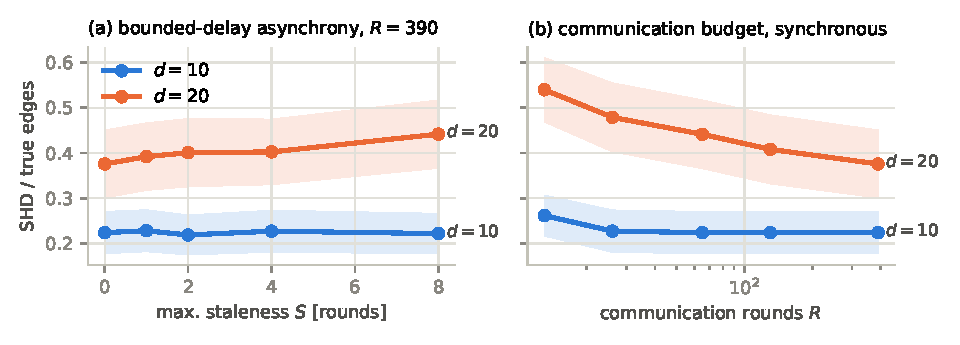
\includegraphics[width=\linewidth]{figures/delay}
\caption{Effect of communication on accuracy ($K=4$ clients, ER3-p1 and SF3-p1, $n=1000$,
mean $\pm$ s.e.m.\ over 10 instances per $d$). (a)~Bounded-delay asynchrony: each client
starts from a model up to $S$ rounds old. (b)~Synchronous \feddbn{} with a budget of
$R$ communication rounds, obtained by varying the number of epochs.}
\label{fig:delay}
\end{figure}

\begin{table}[t]
\centering
\caption{Wall-clock time model \eqref{eq:wallclock} [s]: measured parallel compute time plus
$R(2\ell+16md/\beta)$ for networks with (latency $\ell$, bandwidth $\beta$) = datacentre
(0.1\,ms, 10\,Gb/s), LAN (1\,ms, 1\,Gb/s), WAN (50\,ms, 100\,Mb/s) and cross-continent
(150\,ms, 20\,Mb/s).}
\label{tab:comm}
\small
\begin{tabular}{l r r rrrr}
\toprule
instance & rounds & compute [s] & datacentre & LAN & WAN & cross-continent \\
\midrule
ExDBN bench., $d{=}25$, $K{=}8$ & 390 & 1.0 & 1.1 & 1.9 & 40.7 & 121.1 \\
scaling, $d{=}100$, $K{=}8$ & 130 & 0.9 & 1.0 & 1.5 & 17.2 & 56.6 \\
scaling, $d{=}1000$, $K{=}8$ & 130 & 111.1 & 114.4 & 144.6 & 456.9 & 1814.1 \\
\bottomrule
\end{tabular}

\end{table}

\Cref{fig:delay}(b) shows that the number of rounds matters more than delays. On $d=20$,
13 rounds (one epoch) give a 40--50\% higher SHD than 390 rounds. On $d=10$, 26
rounds already suffice. Bounded staleness, panel (a), is harmless at $d=10$. At $d=20$ it costs
up to 11 SHD on ER3-p1 ($S=8$) but little on SF3-p1. For small models latency dominates the communication cost
(\cref{tab:comm}). On the \exdbn{} benchmark a WAN deployment adds about 40\,s to about one
second of computation. That is still less than the 120\,s the MIP spends in branch-and-bound,
which does not even include gathering the Gram matrix. For $d=1000$ a message has
$md=2\cdot 10^6$ floats (16\,MB), and on slow links bandwidth dominates. A cross-continent
deployment would spend 30 minutes communicating in 130 rounds, so compressing or
sparsifying the updates matters at this scale. In every setting the number of rounds,
not the delay per round, is the quantity to economise.

\subsection{Scalability}
\label{sec:exp-scaling}

\exdbn's generator does not produce instances beyond $d\approx 25$ (\cref{app:details}), so
for scaling we use our own generator for the same model class. It draws an ER intra-slice DAG
with expected degree 4 and one lag with $d$ entries, which gives about $3d$ true edges, with
$n=\max(1000,4d)$, $d$ from 10 to 1000 and three seeds. \feddbn{} runs 130 rounds (10
epochs of 20 local steps). \exdbn{} runs in the Gram form with 120\,s and four threads for
$d\le 250$, and in its original formulation for $d\le 25$ (and for $d=50$ on seed 0, run
alone). \Cref{fig:scaling,tab:scaling}
give the results.

\begin{figure}[t]
\centering
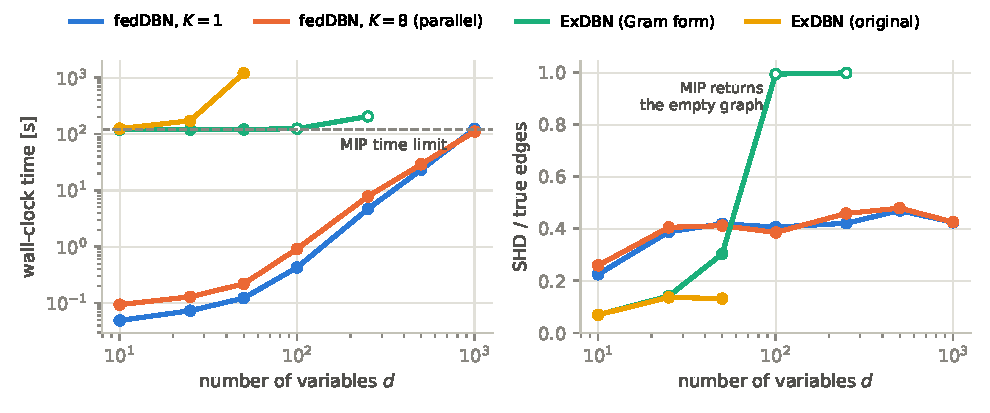
\includegraphics[width=\linewidth]{figures/scaling}
\caption{Scaling on ER instances with one lag and $n=\max(1000,4d)$, mean over three seeds
(one seed for $K=8$ at $d=1000$ and for the original \exdbn{} formulation at $d=50$). Left: wall-clock time. For \feddbn{} this is the parallel
time; for \exdbn{} it is the total time including model building, with the 120\,s limit
dashed. Right: SHD relative to the number of true edges. Hollow markers: the MIP returned the
empty graph.}
\label{fig:scaling}
\end{figure}

\begin{table}[t]
\centering
\caption{Scaling, mean over three seeds (one for $K=8$ at $d=1000$). ``edges'' counts the
true edges in $W$ and $A$. \feddbn{} times are parallel times. \exdbn{} in the Gram form has
a 120\,s limit and four threads. A gap $\gg1$ means that the dual bound is still the trivial
one implied by $|w|\le M$. ``build'' is the time to construct the Gram-form model, and
``orig.'' is the original formulation, with its total time including model building.
$^\dagger$Seed 0 only.}
\label{tab:scaling}
\small
\setlength{\tabcolsep}{4pt}
\begin{tabular}{rr rrr rrr rrrr rr}
\toprule
 & & \multicolumn{3}{c}{\feddbn, $K{=}1$} & \multicolumn{3}{c}{\feddbn, $K{=}8$} & \multicolumn{4}{c}{\exdbn{}, Gram form} & \multicolumn{2}{c}{\exdbn{}, orig.} \\
\cmidrule(lr){3-5}\cmidrule(lr){6-8}\cmidrule(lr){9-12}\cmidrule(lr){13-14}
$d$ & edges & SHD & F1 & time [s] & SHD & F1 & time [s] & SHD & F1 & gap & build [s] & SHD & time [s] \\
\midrule
10 & 30 & 7.2 & 0.79 & 0.05 & 8.5 & 0.78 & 0.09 & 2.3 & 0.96 & 0.01 & 0.02 & 2.3 & 125 \\
25 & 75 & 29.3 & 0.73 & 0.07 & 30.7 & 0.72 & 0.13 & 10.5 & 0.91 & 0.29 & 0.25 & 10.2 & 173 \\
50 & 153 & 64.3 & 0.70 & 0.12 & 63.2 & 0.71 & 0.22 & 46.3 & 0.78 & 0.39 & 0.81 & 20.0$^\dagger$ & 1205$^\dagger$ \\
100 & 303 & 124.0 & 0.73 & 0.43 & 117.8 & 0.75 & 0.92 & 301.7 & 0.00 & $\gg 1$ & 4.80 & -- & -- \\
250 & 771 & 324.5 & 0.73 & 4.65 & 354.2 & 0.72 & 7.80 & 770.0 & 0.00 & $\gg 1$ & 85 & -- & -- \\
500 & 1500 & 705.0 & 0.71 & 23 & 719.0 & 0.67 & 29 & \multicolumn{4}{c}{not attempted} & -- & -- \\
1000 & 2983 & 1267.3 & 0.75 & 124 & 1282.5 & 0.76 & 111 & \multicolumn{4}{c}{not attempted} & -- & -- \\
\bottomrule
\end{tabular}

\end{table}

\textbf{\feddbn's accuracy does not degrade with $d$.} From $d=25$ to $d=1000$ its SHD
stays between 0.39 and 0.48 of the true edges and its F1 between 0.67 and 0.76, for both $K=1$
and $K=8$. Federation costs little at every size: the relative SHD of $K=8$ and $K=1$
differs by at most 0.04.

\textbf{\feddbn's running time is polynomial and predictable.} It grows from 0.05\,s at
$d=10$ to 124\,s at $d=1000$ for $K=1$. A local step multiplies the $m\times m$ Gram matrix
by the $m\times d$ iterate, which costs $O(d^3)$ flops. The measured time grows as
$d^{2.4}$ between $d=250$ and $d=1000$. For $K=8$ at $d=1000$ the parallel time is 111\,s
and the sequential time 761\,s. Each client's local step costs as much as a centralised step,
whatever $n_k$, because it uses an $m\times m$ Gram matrix. Federation therefore brings data
locality, not a speed-up. For $d\le 250$ the parallel time of $K=8$ is 1.7--2.1 times that
of $K=1$, partly because each round waits for the slowest of eight clients.

\textbf{The MIP stops returning useful graphs at $d=100$.} Up to $d=50$, \exdbn{} is clearly
more accurate than \feddbn: its relative SHD is 0.07, 0.14 and 0.30, against 0.23, 0.39 and
0.42 for \feddbn{} with $K=1$. Over the same range its gap grows from 0.01 to 0.39. At
$d=100$ (19\,900 binaries) it returns exactly the empty graph on all three seeds. Its
incumbent is $\Theta=0$, with objective $\operatorname{tr}(S_{XX})$, and its dual bound is
$-8\cdot10^{9}$. On seed 0, Gurobi's log shows that the \emph{root relaxation} hit the time
limit after $6.8\cdot10^4$ simplex iterations in a 45\,s run, and the 120\,s run ends with the
same bound. This convex
QP has $4\cdot10^4$ variables and $2\cdot10^6$ quadratic terms, and the sequential solver
does not solve even this one node. That is the bottleneck of \cref{sec:mip}, reason~3, in its
plainest form. At $d=250$ building the Gram-form model alone takes 85\,s, and the result is
again the empty graph. Within this budget the crossover therefore lies between $d=50$ and
$d=100$. Beyond it, \feddbn{} is the only one of the two methods that returns a graph, with
SHD about 0.4 of the true edges.

\textbf{The original formulation is limited by model building.} It is as accurate as the
Gram form at $d\le 25$ (relative SHD 0.07 and 0.14), but its total time is 125\,s at $d=10$
and 173\,s at $d=25$. That is about 50\,s of model construction on top of the time limit, and the
number of terms to construct grows as $n d m^2$ (\cref{sec:mip}). At $d=50$ (seed 0) the
build takes about 1085\,s, eighteen minutes, and peaks at 12.3\,GB of memory. In its 120\,s
of branch-and-bound this run then found a much better graph than the Gram form on the same
instance: SHD 20 and F1 0.92, against 56 and 0.72, with a similar gap (0.35 against 0.39).
\feddbn{} reaches 60.5 ($K=1$) and 62 ($K=8$) on this instance. The two formulations define the
same optimisation problem, so the difference reflects how sensitive a time-limited
branch-and-bound is to presolve and search order, and to the fact that this run had the
machine to itself. One instance is not enough to say more. It does show that the ranking up
to $d=50$ favours the MIP, \emph{if} one can afford to build the model.

\section{Discussion and limitations}
\label{sec:discussion}

\paragraph{Where the price comes from.}
The breakdown is unambiguous. Federation in the narrow sense, that is splitting the data
and averaging local models, costs little: under 2 SHD for $K=8$ on average, and it is
explained by client drift when clients hold fewer time points than there are regressors.
Incomplete optimisation is negligible once the order is fixed. Communication delays act
through the number of rounds, and through staleness at $d=20$. Almost the entire price is
\emph{combinatorial}: \psidag's greedy, data-free projection picks a suboptimal
topological order and rarely revises it. With the true order, the same least-squares
estimator is nearly exact. The question ``how much worse is the federated first-order method
than the exact MIP?'' therefore reduces, to first order, to ``how good is the projection's
order?''. Federation is not the issue.

\paragraph{Improving the order.}
Since the ordering term dominates, the most promising improvements of \feddbn{} target the
projection. Options include several restarts selected by the federated loss, which is
embarrassingly parallel and costs one scalar per client per restart; local search over
adjacent transpositions, scored by clients; and projections that account for the scale of
the variables. Any of these must keep the projection free of data, or else pay for it in
communication.

\paragraph{Limitations.}
(i) All clients are homogeneous in distribution, since they hold windows of one stationary series.
Heterogeneous clients (different noise levels or mechanisms) cause client drift
\citep{karimireddy2020scaffold}, and \feddbn{} would then need drift correction.
(ii) We report the SHD at the oracle threshold, as \exdbn{} does. It favours continuous methods,
which do not fix the support themselves. We also store SHD at a fixed threshold of $0.1$ in
the released results.
(iii) \exdbn{} was run with the 120\,s limit of its main experiments, on two threads.
\Cref{tab:budget} shows that its accuracy for $d\ge 20$ is very sensitive to this budget. A
systematic sweep over time limits and threads, and the resulting time to accuracy, is left
for future work. Its worst-case running time is exponential in any case.
(iv) \feddbn{} shares iterates. Iterates of a least-squares problem reveal information about
the clients' Gram matrices, and formal privacy, for example differentially private
aggregation, is future work.
(v) We provide no convergence theory for the federated projection scheme. \citet{ziu2024psi}
analyse the centralised stochastic-approximation iteration. Extending this analysis to local
steps and bounded delays is open.

\paragraph{Conclusion.}
We proposed \feddbn, a federated extension of \psidag{} to dynamic Bayesian networks, and
measured its price of federation against the exact MIP \exdbn{}, which by
\cref{prop:gram} can itself be federated with one round of secure aggregation. The price
is real for small models: about 27\% of the true edges for $d\le 15$. Almost all of it is
due to the greedy order of the projection, not to splitting the data, incomplete
optimisation or communication delays. For larger models the comparison turns around in
practice, even though the MIP remains better in principle. With 120\,s per instance the MIP
is no better than \feddbn{} at $d=20$--$25$. It needs several times more compute to recover
the true graph there, and from $d=100$ on it cannot solve even its root relaxation. \feddbn{}
keeps an SHD of about 0.4 of the true edges up to $d=1000$, at a cost that grows polynomially
and is known in advance. Better data-free projections are the natural next step: they
target the one term that dominates the price.


\bibliography{references}
\bibliographystyle{tmlr}

\appendix
\crefalias{section}{appendix}
\section{Experimental details}
\label{app:details}

\paragraph{Data.}
\exdbn{} instances are produced by \exdbn's own \texttt{load\_problem} with
\texttt{set\_random\_seed(seed)}, exactly as in its \texttt{start\_experiment}. The parameter
tuples $(p,\ \text{intra edge ratio},\ w^{\min}_{\mathrm{inter}},\ w^{\max}_{\mathrm{inter}},\ \text{noise scale})$
are ER3-p1 $=(1,3,0.2,0.4,1.0)$, SF3-p1 $=(1,3,0.2,0.4,1.0)$ with a Barab\'asi--Albert
intra-slice graph, and ER2-p2 $=(2,2,0.3,0.5,1.0)$. Intra-slice weights are uniform on
$\pm[0.5,2]$ and lag weights decay by a factor $1.1$ per lag. \exdbn's generator rejects
series whose magnitude exceeds $10^3$ and gives up after 1000 attempts. Where it gives up, the
instance is skipped, as in \exdbn's own experiment script. This happens for all ER2-p2
instances with $d\ge 15$ except one (ER2-p2, $d=15$, $n=1000$, seed 3) and for ER3-p1 with
$d=25$, $n=1000$, seed 0. ER3 graphs with $d=5$ do not exist, since $3d$ edges exceed
$\binom52$. Of the 150 grid points, 110 instances remain.
The scaling instances use \psidag's DAG generator (ER, expected degree 4, weights
$\pm[0.05,1]$) for $W$, \exdbn-style lag matrices ($d$ entries, $|a|\in[0.2,0.4]$), a
stability rescaling of $A$ so that the reduced-form VAR has spectral radius at most $0.9$,
$n=\max(1000,4d)$ and a burn-in of 200 steps.

\paragraph{Clients.}
The rows $(x_t, x_{t-1},\dots,x_{t-p})$ are split into $K$ contiguous, disjoint time windows of
equal length. Clients are therefore homogeneous in distribution, but each sees only $n/K$
time points: 31 points per client for $n=250$ and $K=8$.

\paragraph{fedDBN hyperparameters.}
On the \exdbn{} benchmark: $E=30$ epochs, $R_u=3$, $R_c=10$ (390 rounds), $T=100$ local
steps, exact local gradients, Nesterov momentum $0.95$, step $1/L_k$, no $\ell_1$ penalty.
These values were chosen on separate tuning instances (seeds 100--104, ER3-p1 with $d\in\{10,20\}$)
among a handful of candidates, and then frozen. For scaling: $E=10$, $T=20$ (130 rounds) and
otherwise the same.

\paragraph{\exdbn{} settings.}
We use \exdbn's \texttt{solve\_milp.solve} unchanged ($\lambda_1=\lambda_2=0.1$,
$M=100$, MIP gap $10^{-4}$, lazy constraints for all cycles found in an incumbent) with a
time limit of 120\,s, as in \exdbn's main experiments, and 2 Gurobi threads per run with
3--4 runs in parallel. The Gram form (\cref{prop:gram}) uses the same settings. In the
scaling experiment it uses 4 threads, with two runs in parallel. The budget check of
\cref{tab:budget} solves its four instances one after another, with 2 or 6 threads.
Gurobi 12.0.3 ran on an Apple M2 Pro (10 cores, 32\,GB). \feddbn{} uses PyTorch with one
thread per process, and clients are simulated sequentially. We report the \emph{parallel}
time: the slowest client per round, plus the server's projections, plus the slowest client's
setup.

\paragraph{Metrics.}
We use \exdbn's evaluation code (\texttt{find\_optimal\_threshold\_for\_shd},
\texttt{count\_accuracy}) on the \exdbn{} benchmark, and an exactly matching vectorised
re-implementation for $d>25$, where the original pure-Python code is too slow. On the
scaling instances the oracle threshold is searched over 400 quantiles of the estimated
$|$weights$|$. F1 is the standard entrywise F1 on the stacked support $[W;A_1;\dots;A_p]$, so a
reversed edge counts as one false positive and one false negative. \exdbn's SHD charges
$\tfrac12$ for a reversed pair and, for the lag matrices, compares unordered pairs
$\{i,j\}$, $i>j$, so self-lag entries are not part of the SHD.


\end{document}
